Low-Earth-orbit (LEO) satellite constellations rely on uniform angular
spacing between spacecraft to provide continuous ground coverage.
In a nominally equally-spaced constellation of $N$ satellites on a
common circular orbit, adjacent satellites are ideally separated by
$360^{\circ}/N$.

In practice, perturbations---atmospheric drag, Earth's $J_2$
oblateness term, and solar radiation pressure---shift each
satellite's argument of latitude at a different rate. Left uncorrected,
the spacing drifts and coverage gaps emerge. Periodic \emph{phasing
manoeuvres} must therefore restore equal spacing.

\begin{figure}[H]
  \centering
  \begin{minipage}[t]{0.46\linewidth}
    \centering
    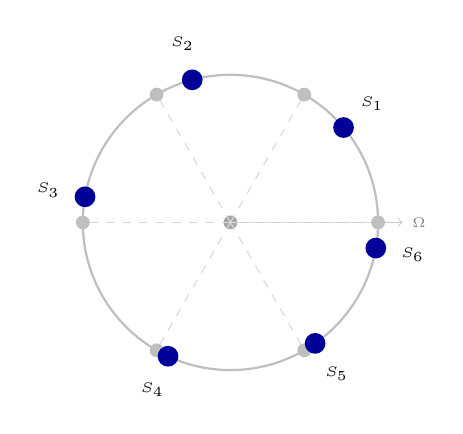
\begin{tikzpicture}[scale=1.25]
      \draw[thick, gray!50] (0,0) circle (1.5);
      \fill[gray!70] (0,0) circle (0.07);
      \draw[->, gray!40] (0,0) -- (1.75,0)
        node[right, font=\tiny, gray]{$\Omega$};
      % ideal equally-spaced slots
      \foreach \k in {0,...,5}{
        \draw[gray!30, dashed, thin] (0,0)
          -- ({1.5*cos(60*\k)},{1.5*sin(60*\k)});
        \fill[gray!50] ({1.5*cos(60*\k)},{1.5*sin(60*\k)}) circle (2pt);
      }
      % perturbed satellites
      \foreach[count=\i] \a in {40,105,170,245,305,350}{
        \fill[blue!60!black] ({1.5*cos(\a)},{1.5*sin(\a)}) circle (3pt);
        \node[font=\tiny] at ({1.88*cos(\a)},{1.88*sin(\a)}) {$S_{\i}$};
      }
    \end{tikzpicture}\\[3pt]
    {\footnotesize (a) Non-uniform initial spacing.}\\[2pt]
    {\small\textcolor{blue!60!black}{$\bullet$}~current\quad
           \textcolor{gray!60}{$\bullet$}~ideal slot}
  \end{minipage}
  \hfill
  \begin{minipage}[t]{0.46\linewidth}
    \centering
    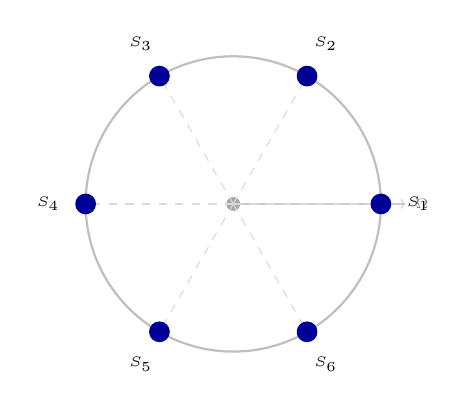
\begin{tikzpicture}[scale=1.25]
      \draw[thick, gray!50] (0,0) circle (1.5);
      \fill[gray!70] (0,0) circle (0.07);
      \draw[->, gray!40] (0,0) -- (1.75,0)
        node[right, font=\tiny, gray]{$\Omega$};
      % equally spaced after manoeuvres
      \foreach[count=\i] \a in {0,60,120,180,240,300}{
        \draw[gray!30, dashed, thin] (0,0)
          -- ({1.5*cos(\a)},{1.5*sin(\a)});
        \fill[blue!60!black] ({1.5*cos(\a)},{1.5*sin(\a)}) circle (3pt);
        \node[font=\tiny] at ({1.88*cos(\a)},{1.88*sin(\a)}) {$S_{\i}$};
      }
    \end{tikzpicture}\\[3pt]
    {\footnotesize (b) Equal $60^{\circ}$ spacing after manoeuvres.}
  \end{minipage}
  \caption{Six-satellite LEO constellation viewed from above (ascending
    node $\Omega$ to the right). Grey dots in~(a) mark the six ideal
    equally-spaced positions; coloured dots show actual satellite
    locations. After two-burn phasing manoeuvres each satellite occupies
    a slot and the constellation is restored to uniform spacing~(b).}
  \label{fig:intro:constellation}
\end{figure}

Each manoeuvre consumes propellant, and the remaining fuel budget
determines a satellite's remaining operational lifetime. Because
perturbation rates differ between spacecraft, budgets can become
unequal over time, so balancing remaining fuel across the fleet is
as important as minimising total consumption.

This work presents a \MATLAB{} implementation that, given the current
arguments of latitude and $\dv$ budgets of an $N$-satellite constellation,
finds the cheapest set of two-burn phasing manoeuvres that restores equal
spacing. Two multi-objective strategies are implemented and compared:
\begin{itemize}
  \item a \textbf{weighted-sum} strategy, which combines total $\dv$
        consumption and fuel imbalance into a single scalar objective;
  \item a \textbf{lexicographic} strategy, which minimises total fuel
        consumption first and then minimises imbalance subject to the
        optimal consumption value.
\end{itemize}

The source code is publicly available at
\texttt{github.com/EdwardEisenhauer/AAE-NMaO}.
